\documentclass[a4paper,oneside]{scrarticle}

\usepackage[left=3cm,right=3cm,top=2cm,bottom=2.25cm]{geometry}
\usepackage[ngerman]{babel}
\usepackage{amsmath}
\usepackage{amsfonts}
\usepackage{amssymb}
\usepackage{mathtools}
\usepackage{graphicx}
\usepackage{hyperref}
%\graphicspath{ {./images/} }
\addto\captionsngerman{\renewcommand{\figurename}{Fig.}}


\begin{document}
	\begin{flushleft}
		Bach Nguyen, Johannes Roloff - HTWK Leipzig - INB
	\end{flushleft}

	\begin{center}
		\begin{LARGE}
			\textbf{Station 1 Zielsetzung}
		\end{LARGE}
	\end{center}
	\section*{Einordnung der Aufgabe im Prozess}
	\begin{figure} [h]
		\centering
		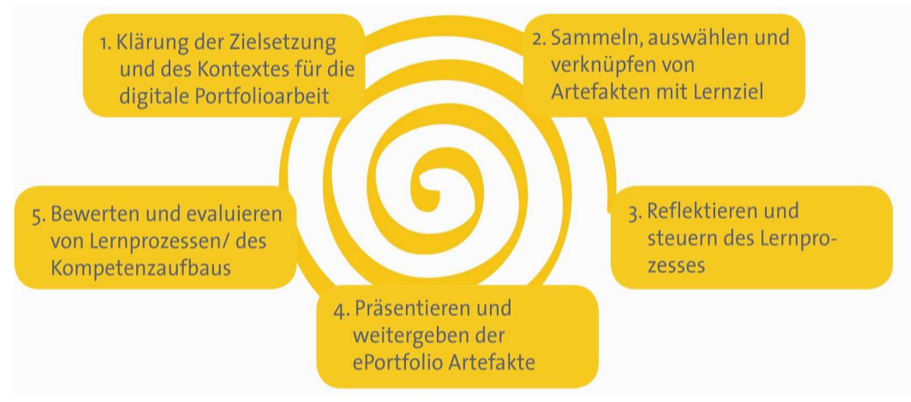
\includegraphics[width=0.7\linewidth]{e-portfolio-prozesse-schaffert}
		\caption{Prozesse der Portfolio-Arbeit (Schaffert et al. 2007, S. 79)}
		\label{fig:e-portfolio-prozesse-schaffert}
	\end{figure}
	\begin{figure}[h]
		\centering
		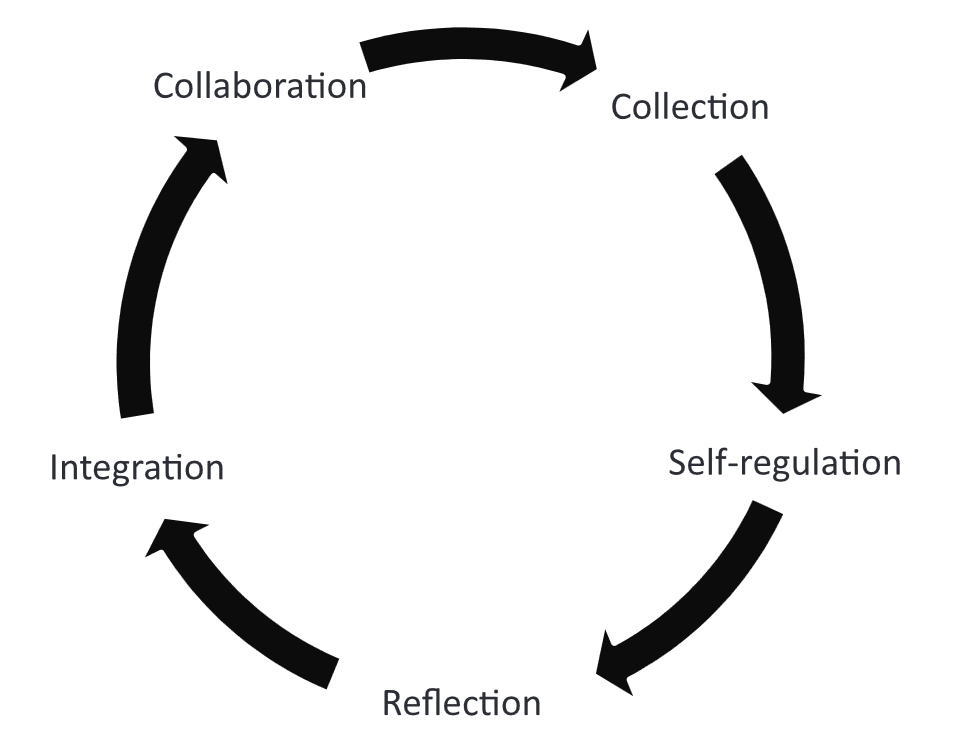
\includegraphics[width=0.5\linewidth]{cycle-of-documented-lifelong-learning-Jensen}
		\caption{cycle of documented lifelong learning (Jensen,Treuer 2014)}
		\label{fig:cycle-of-documented-lifelong-learning-jensen}
	\end{figure}
	\begin{figure}[h]
		\centering
		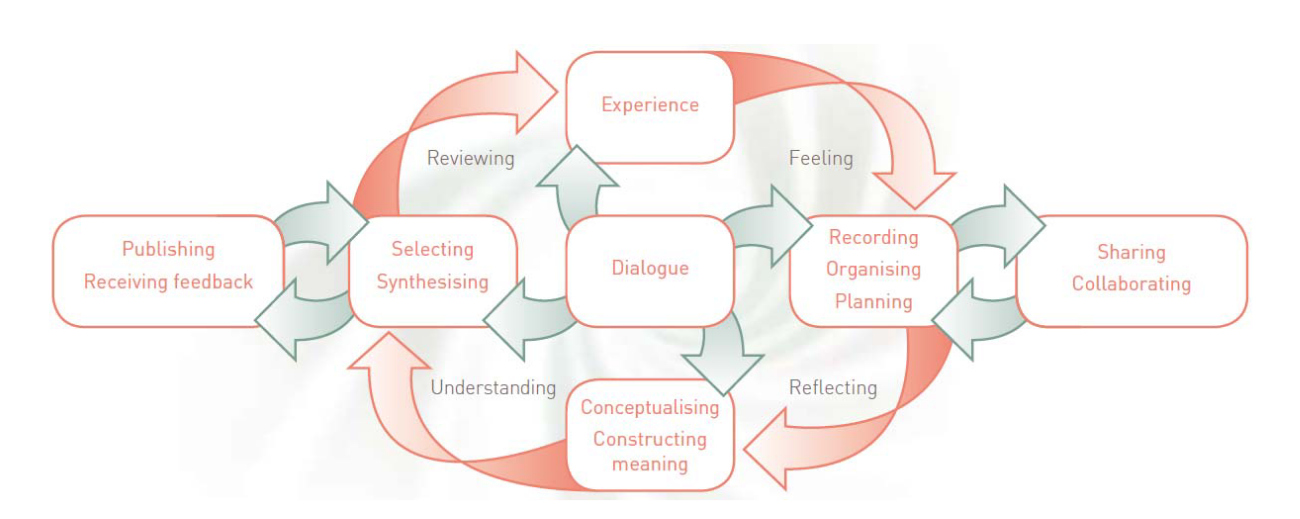
\includegraphics[width=0.8\linewidth]{model-of-e-portfolio-based-learning}
		\caption{A model of e-portfolio-based learning (JISC 2008, S. 9)}
		\label{fig:model-of-e-portfolio-based-learning}
	\end{figure}

	\pagebreak 
	
	\section*{Informationsmaterialien}
	Lese dir diesen \href{https://www.atlassian.com/blog/productivity/how-to-write-smart-goals}{Artikel} durch zu SMARTen Zielen und behalte diese Ideen im Überblick bei der Erstellung deiner Ziele.\\
	
	\bibliographystyle{alpha}
	\bibliography{../eportfolio_lib}
	
	
	\pagebreak
		
	\section*{Einleitung}
	Was bedeutet das Zielsetzen. Und wozu brauchen wir E-Portfolios? Was sind SMART goals?
	
	\section*{Aufgabenstellung}

	\begin{enumerate}
		\item Was möchtest Du mit deinem E-Portfolio erreichen?
		\item Stelle dir vor Du würdest erst nächste Woche anfangen mit einem Modul deiner Wahl in einem der vorhergehenden Semester. Schreibe deine Vorstellungen an das Modul und nutze auch Modulux für mögliche Lernziele. Versuche an dieser Stelle mindestens folgende Fragen zu beantworten:
		\begin{enumerate}
			\item Was möchte Ich am Ende des Moduls nach der Prüfung für Mich selbst mitgenommen haben?
			\item Wie viel Zeit möchte Ich in dieses Modul stecken in jeder Woche?
		\end{enumerate}
		\item Stelle dir vor Du würdest erst nächste Woche anfangen mit diesem Bachelor Studium. Schreibe deine Vorstellungen an das Studium und versuche an dieser Stelle mindestens folgende Fragen zu beantworten:
		\begin{enumerate}
			\item Was möchte Ich am Ende des Studiums nach der Prüfung für Mich selbst mitgenommen haben?
			\item Wie viel Zeit möchte Ich in dieses Studium stecken in jeder Woche?
			\item Was möchte Ich außerhalb der akademischen Rahmens geschafft haben?
		\end{enumerate}

	\end{enumerate}


\end{document}
